\documentclass[12pt]{article}
\usepackage{authblk}
\usepackage{titling}
\usepackage{lipsum}
\usepackage{graphicx}
\usepackage{listings}
\lstset{frame=tb,
  language=Python,
  aboveskip=3mm,
  belowskip=3mm,
  showstringspaces=false,
  columns=flexible,
  basicstyle={\small\ttfamily},
  numbers=none,
  numberstyle=\tiny\color{gray},
  keywordstyle=\color{blue},
  commentstyle=\color{dkgreen},
  stringstyle=\color{mauve},
  breaklines=true,
  breakatwhitespace=true,
  tabsize=3
}
\title{Implementation and evaluation of four different Byzantine Reliable Broadcast protocols}
\author{Gianmarco Bordin, Gabriele Lerani, Carlo Giralda}
\affil{Department of Engineering in Computer Science, \\ Sapienza Università di Roma}
\date{June 2023}

\begin{document}
\maketitle
\begin{abstract}
This paper examines four byzantine reliable broadcast protocols along with their implementation and provides a performance evaluation of them. At this time, the importance of efficient protocols that can guarantee byzantine reliable broadcast's properties is raising up due to the growth of the internet communication world and the centrality of cyber security goals with respect to byzantine processes. 
\end{abstract}

\newpage

\section{Summary}

1. Introduction\\
2. Assumptions\\
3. Initialization and Installation\\
4. Description of the protocols\\
5. Implementation\\
6. Simulation

\newpage

\section{Introduction}

A Byzantine fault is a condition of a computer system, particularly distributed computing systems, where components may fail and there is imperfect information on whether a component has failed.\\ The term takes its name from an allegory, the "Byzantine generals problem", developed to describe a situation in which, in order to avoid catastrophic failure of the system, the system's actors must agree on a concerted strategy, but some of these actors are unreliable.\\
In a Byzantine fault, a component such as a server can inconsistently appear both failed and functioning to failure-detection systems, presenting different symptoms to different observers. It is difficult for the other components to declare it failed and shut it out of the network, because they need to first reach a consensus regarding which component has failed in the first place. Byzantine fault tolerance (BFT) is the resiliency of a fault-tolerant computer system to such conditions.\\
In this context the byzantine reliable broadcast specification guarantees the following properties:\\
1) Validity: If a correct process p broadcasts a message m, then every correct process eventually delivers m;\\
2) No duplication: Every correct process delivers at most one message;\\
3) Integrity: If some correct process delivers a message m with sender p and process p is correct, then m was previously broadcast by p;\\
4) Consistency: If some correct process delivers a message m and another correct process delivers a message m' then m = m'.

\newpage

\section{Assumptions}

In our implementation we assumed the following: \\
- Each process connects to a bootstrap server to gather its unique ID:\\
- The server(s) address(es) is(are) known to every process in the network; \\
- Every process knows the ID of the broadcaster that is settled to one in our implementation; \\
- The broadcaster brodacasts the message only to processes that it knew about before the broadcast primitive, so subsequent receivers, that connect to the service afterwards, will not receive it; \\
- The network is fully connected; \\
- In the Bracha code Algorhtm, every array that contains messages of a specific type is checked according to an interval of time (e.g every .001 s); \\
- The message is considered delivered when the "- - - - -Message Delivered - - - - -" string is prompted in the terminal; \\
- All the algorithms use SHA256 cryptographic hash function; \\
- Authenticated Messages code algorithm uses the ‘RSA’ API interface in order to make the digital signatures; \\
- Erasure Code algorithm uses the ‘pyeclib’ API interface in order to derive the shares; \\
- A faulty process is a process that discards every message that it receives after the time it fails; \\
- Erasure Code algorithm considers the "source" field of a message instead of the "from" message field for finality and soundness reasons; \\
- Byzantine processes are modeled with specific python modules. \\

\newpage

\section{Initialization and installation}

Our implementation of the protocols requires at least python 3.10.
These are the following commands needed to run the algorithms implementation on the python environment:
\begin{lstlisting}
pip install -r requirements.txt
\end{lstlisting}
Also it is required to install docker,rabbitmq from the official sites and running the following in the docker prompt:
\begin{lstlisting}
docker start
docker run -d -p <ip_address>:5672:5672 -p 15672:15672 rabbitmq:3.8.15-rc.2-management
\end{lstlisting}
To run the simulations it is necessary to install the onos controller with:
\begin{lstlisting}
sudo docker run -t -d -p 8181:8181 -p 8101:8101 -p 5005:5005 -p 830:830 --	name onos onosproject/onos
\end{lstlisting}
We used mininet as a simulation environment so if you want to run the simulation.py script you need to run sudo bash first.\\

\newpage

\section{Description of the protocols}
In this section will be stated all the four protocols implemented and considered in the simulations.
\\
\subsection{Authenticated Links(AL)}
This protocol takes advantage of the underlying authenticated link primitive between each pair of processes to exchange messages for guaranteed authenticity of the processes.The protocol specification is structured in this way:\\
In The first phase the sender broadcasts a message to all other processes in the network through a SEND message.\\
In the second phase, when a process receives a SEND message from the broadcaster, it sends to every process an ECHO message. So each process stores these messages to count them.\\
As soon as a process counts to (N+f)/2 +1 ECHO messages for the same message m, it enters phase three.
In the third phase each process that has received (N+f)/2+1 ECHO messages for a specific message m,broadcasts to all other processes a READY message and as soon as it receives a READY message it stores it. \\If a process counts to f+1 READY messages for the same message m it re-broadcasts them to all others.  If a process counts to 2f+1 READY messages for the same message m and it has not already delivered that message m, it can deliver it. \\
\\
\subsection{Authenticated Messages(AM)}
This protocol takes advantage of the digital signature to digitally sign messages sent from a specific node for guaranteed authenticity and non-repudiation. \\The protocol specification is structured in this way:\\
Propose-Phase. The designated broadcaster L with input v sends ⟨propose, v⟩ to all parties.\\
Vote-Phase. When receiving the first proposal ⟨propose, v⟩ from the broadcaster, send a vote message for v to all parties in the form of ⟨vote, v⟩i .\\
Commit-Phase. When receiving n minus f signed vote messages for v, forward these vote messages to all other parties, commit v and terminate. \\
\\
\subsection{Hash-Based(HB)}
This protocol takes advantage of the cryptographical hashing.In particular, the correctness of the algorithms rely on the collision-resistant property of the hash function used. Cryptographic hash functions are used widely in real-world applications.The protocol specification is structured in this way:\\
The source node simply sends a MSG message containing its identifier, message content m, and the sequence number h, to all the nodes. Following the convention, we assume that the source also sends the message to itself. Each node may receive five types of messages: \\
– MSG message: this must come directly from the source which contains the message content m. If the source identifier does not match the sender identifier, then the message is discarded. \\
– ECHO message: this message propagates information about a message already received by some node. ECHO messages contain the full content m. In the hash based algorithms, we only transmit H(m). This is the main reason that we are able to reduce bit complexity. \\
– ACC message: this message is used to declare to other nodes when a certain node is ready to accept a message m. Again, instead of sending m with the ACC message, we send H(m). \\
– REQ messages: In our hash based approach, a node might not know the original message m, even after it has observed enough ACC(m) messages supporting it. Therefore, such a node needs to use a REQ(H(m)) message to fetch the original message content from some non faulty node before accepting it. \\
– FWD messages: When a node is sent a REQ(H(m)) message, it replies with a FWD(m) message that contains the original message content of m. \\
\\
\subsection{ Erasure Code Based(EC)}
This protocol takes advantage of the erasure coding technique that makes possible to decompose a message into shares and its reconstructions knowing a sufficient number of shares.The protocol specification is structured in this way:
EC will use [n, k] MDS code. To send a message m with sequence number h, it encodes the message m and then disseminates to each peer. The message is a tuple that contains the tag MSG, the source identifier s, corresponding coded element, and sequence number of the message h. To deal with asynchrony and failures, the algorithm is event-driven. First, upon receiving a coded element from the source, node i forwards an ECHO message along with the coded element. Second, upon receiving an ECHO message, node i decodes the message if it has received enough coded elements. The key design behind how crash-tolerant RB achieves the all-or-nothing property is that each peer needs to (pessimistically) help deliver the message to other peers. \\

\newpage

\section{Implementation}
In this section we focus on the implementation choices regarding the four algorithms stated in the previous section.
The architecture of all the procols is mainly organized in three modules:
    – The server module(Server.py)
    – The process module(Process.py)
    – The authenticated link module(AuthenticatedLink.py) \\
\\
\subsection{Authenticated links}
We now describe the python modules for the implementation of the Al protocol. This protocol uses the authenticated link primitives to ensure authenticity. \\
\subsubsection{Server.py}
In the server module we have the bootstrapping functions required to assign to every process a unique id. The id is pushed in a rabbitmq together with the ip address of the process receiving that id, so every process receives in its queue the list of the active processes as the form <IP,ID>. The id is created following a simple auto increment policy. Every time that a new process connects to the server to gather its id, the server module creates a new serving thread for this connection and delegates to it the management of the new client request. Subsequently another thread pushes the  new pair <IP,ID> inside every active process queue.For efficiency concerns all the queues are deleted after an inactivity timeout: realized in the implementation through the functions "delete queues","on timeout", "start counter". \\
\subsubsection{Process.py}
In the process module we have the implementation of the real byzantine reliable broadcast primitives. As a first step the function “connection to server” make the process open a socket to connect to the bootstrap server mentioned above to gather ids information and subsequently starts a thread that has the task to check if for a subset of the messages received and stored some delivering or forwarding condition holds.Every process reads the ids of the active processes through a rabbitmq structure using the “pika” library in the “update function”.\\ After that every process stores the ids and the Ips of all the processes in two lists indexed coherently to the order of the processes' connections. The latter step is to call the “creation links” function that is in charge of instantiating the underlying authenticated links module and subsequently to store the references to these modules in a list.\\ After the creation of the links this function calls for every entry of the authenticated links list, the function “receiver” described in the following section”.\\
After these initialization steps the broadcaster process can call the broadcast function to send a message to every process in the network. Firstly it calls its own “update” function to update its view of the network gathering new network joining processes ids. 
Secondly it uses the underlying module to send to every process a message using the “send” authenticated links function.\\
Each process has a callback function that allows the underlying module to call it after a message for it has been received by the authenticated link module.\\
The “deliver send”,”deliver echo”,”deliver ready” functions make the process store the messages with the related flags in a list called “currentMSG" that lists all the received messages. Every time a process receives a message with a specific flag the related dictionary containing for every key(id) a value(message received) is updated if the message is valid. \\In the listening thread function, the thread that runs this function counts how many values every message flag dictionary contains, for efficiency concerns this parsing is repeated after a sleeping time :"BREAK TIME" in the implementation. If the counters satisfy a different condition a specific action is taken according to the algorithm. So the process can deliver the message if it has counted sufficient numbers of ready messages from the other processes. \\
\subsubsection{AuthenticatedLinks.py}
This module has the task to create a logical authenticated channel between every pair of processes that participates in the network.The message is implemented as a dictionary containing:\\
- the message;\\
- the flag;\\
- the fingerprint;\\
The messages are serialized and loaded according to the json APIs.
The socket addresses are created according to a combination of the ips and ids of the two processes involved in the exchange. 
This module takes as input of the constructor: \\
- the reference to the upper module process.py;
- the id of the receiving process namely the pair (IP,ID);
- the address of the sending process namely the pair (IP,ID).\\
Thanks to these params the authenticated links module can correctly create a socket pair for the calling process.\\
In the function "receive" the thread that runs on it,instantiated in the "receiver" function called by the upper module,creates the socket for receiving the messages coming from another process and calls the "add key"to store the new authentication key for this channel. After storing the new key the function calls the "deliver" function that after checking the authentication of the message it calls the related upper module "deliver(FLAG)" function according to the value of the variable "(FLAG)".
When a process wants to send a message it calls the "send" function that after creating the sending socket, creates the fingerprint of the message and the authentication key if it was not already created. The fingerprint is created with the hashlib.sha256 function instead the authentication key for the channel is created with the "generate key" function of the cryptography library. \\
\\
\subsection{Authenticated Messages}
We now describe the python modules for the implementation of the AM protocol. This protocol uses the digital signature primitives to guarantee non-repudial. \\
\subsubsection{Server.py}
The server module is analogous to the server.py of the previous algorithm description. \\
\subsubsection{Process.py}
The "connection to server", "creation links","update" and the broadcast function are analogous to the previous algorithm. After setting up a vision of the network with the above described functions, a process broadcasts a message using the broadcast function, but before it has to generate its key pair using the "get key pair" function and it has to get the keys of the other processes participating in the protocol using the "get process keys" function, connecting to the KDS.
This is the main module of the implementation; it uses two link primitives following the algorithm specification. In the first phase the broadcaster broadcasts to all the "PROPOSE" flagged messages using the authenticated links primitive without signing the message.
In the second phase every process can send a "VOTE" flagged message using the RSA digital signature and using the Link module.
When a process wants to send a "VOTE" flagged message it calls the "make signature" function that signs the pair (message,flag); here, the "TYPE" flag is used to distinguish between the above-mentioned phases of the algorithm. When a "VOTE" message arrives from the lower module through the callback "process receive" function, each process must check the message signature using the related stored key in the "check signature" function. Every message that is valid is stored in the "vote signed mess" through the "check" function and the related structure of "counter signed messages" is incremented accordingly. The module also uses a "checked" dictionary to verify if a pair (message,related signature) has been already checked to increase performance. The "counter signed messages" is implemented as a dictionary with the message as key attribute and the incremental value of the counter as the value; the "vote signed mess" is implemented as a list of messages(dictionaries). In the final part of the algorithm if a process has to forward its n-f valid "VOTE" messages for a message m it uses a "vote messages" dictionary sent using the underlying link module; the "vote messages" dictionary contains the list of the valid signed messages for that specific message m. \\
\subsubsection{AuthenticatedLinks.py}
The authenticated links module is analogous to the server.py of the previous algorithm     description apart from the condition to stop listening to the receiving socket channel where the connection is closed when a message of type "PROPOSE" is received, according to the fact that after the first phase of the algorithm when the broadcaster has sent a "PROPOSE" message to all processes using the authenticated primitive, every process does not reuse the authenticated links to send messages; instead, every process uses the signed messages in combination with the normal perfect point to point links. When a process message is received by the authenticated link module the "process receive" function of the above described module is called back. \\
\subsubsection{Link.py}
This module has the logical role of instantiating the lower link handler module. It can launch the two threads necessary to manage connections for messages to send to or to receive from other processes. It also has a "link receive" function that has the same role as the above-mentioned protocols: it calls back the upper process module. It uses two flags to make the threads stop when the protocol ends. \\
\subsubsection{Link handler.py}
This module has the trivial function of opening two sockets for receiving/sending messages to the other processes. It also checks if the terminating conditions hold to shutdown the socket pair. \\
\subsubsection{KDS.py}
This module has a similar role to the Server.py module but it distributes the keys necessary to sign the messages and to guarantee authenticity and non-repudiable.
This module simply acts as an always-on key distribution server that attends connections on  a specific port and parses the messages received from the process participating in the network. When a process wants to sign a message it has to generate its private/public key pair so it calls the "handle read" function of the KDS server. This function parses the message received as a dictionary and scans its type to check if the current process has to generate a new key pair or it is asking for the public key of another process in the network to verify a signature. \\
\\
\subsection{Hash Based}
We now describe the python modules for the implementation of the HB protocol. this protocol uses the cryptographical hashing function to ensure integrity. \\ 
\subsubsection{Server.py}
The server module is analogous to the server.py of the previous algorithm description.
\subsubsection{Process.py}
The "connection to server", "creation links","update" and the broadcast function are analogous to the previous algorithm. After setting up a vision of the network with the above described functions, a process broadcasts a message using the broadcast function; The message is firstly packed as a dictionary containing the flag,the message and the sequence number. Like in the previous algorithm there are separated receiving functions depending on the value of the flag of the message parsed by the underlying authenticated links module.\\ Each function is called by the underlying module according to the flag parsed. In this module the "MSGset" is implemented as a dictionary composed of (tuple(message source,message sequence number);list(actual messages received with that key attributes))pairs.\\
The algorithm uses lists containing "echo","acc","req","fwd" flagged messages as structures to verify if a certain message with key attributes has been already received.\\
The algorithm also uses two dictionaries to store the counters for messages received related by the key attributes fields specified in the algorithm specification. The "check" function is called by the receiving function when certain conditions specified in the algorithm implementation occur. To state if a message with key attributes (message,flag,sender) has been already received the implementation uses a "first" function that simply verifies if a certain key (message,flag,sender) exists already in one of the above mentioned lists. \\
\subsubsection{AuthenticatedLinks.py}
The authenticated links module is analogous to the server.py of the previous algorithm description apart from the condition to stop listening to the receiving socket channel where the connection is closed when a message of type "ACC" is received according to the algorithm specification. \\
\\
\subsection{Erasure Code Based}
We now describe the python modules for the implementation of the EC protocol. This protocol uses the erasure-coding techniques to ensure the FEC. The primitive used to create the protocol's shares supports a maximum number of processes; so the simulations are bound to that number (32). \\
\subsubsection{Server.py}
The server module is analogous to the server.py of the previous algorithm description. \\
\subsubsection{Process.py}
As with the previous algorithm we have implemented the message as a dictionary containing the relevant fields like: the flag field, the message field,codicing element field and the Hash field described also in the algorithm specification. For this algorithm we have designed these data structures to implement the different functions required to develop the algorithm:\\
The "msgset" containing all the different messages received by a process is a dictionary with as a key attribute a tuple composed by the message source and the message sequence number and as the value: the list of the messages received with those key attributes.\\
The "codeset" contains all the different coding elements received by a sender with a certain source of the message,hash of the message and sequence number of the message received. The structure designed to implement this is a dictionary with as key attributes the above described identification values and as the value the list of the coding elements concerning those key attributes.\\
The counters ,for the different types of messages received, are implemented as a dictionary that contains incremental counters for messages received by a sender with a certain flag of the message,source of the message,hash of the message and sequence number of the message received.\\ The structure designed to implement this is a dictionary with as key attributes the above described identification values and as the value an incremental integer concerning those key attributes.
To state if a specific flag-labeled message has been already sent/received by the process we have designed dictionaries to contain this information. Each dictionary is indexed according to the key attributes stated in the algorithm specification.\\
The "connection to server", "creation links","update" and the broadcast function are analogous to the previous algorithm. After setting up a vision of the network with the above described functions, a process broadcasts a message using the broadcast function; The message is firstly packed as a dictionary containing the flag,the message and the sequence number. Like in the previous algorithm the are separated receiving functions depending on the value of the flag of the message parsed by the underlying authenticated links module. The underlying module takes as reference for the above process module, the "process receive" function that in turn redirects the flow to the actual receiving process function to do related actions following the algorithm specification.\\
The last function is the "check" function and it is implemented following the specification of the algorithm; to check if a message with a certain hash has been already received by a process, we have implemented a flag, namely "there is", that is set to true when for a certain index "j" exists in the "msgset" dictionary a message "j" that has the same hash value of the received message hash previously computed. For listing all the possible subsets of a set we have used the "get powerset" function that follows a trivial recursion algorithm. \\
\subsubsection{AuthenticatedLinks.py}
The authenticated links module is analogous to the server.py of the previous algorithm.   When a process message is received by the authenticated link module the "process receive" function of the above described module is called back. \\

\newpage

\section{Simulation}
For the simulation part we used mininet with variable number of virtual hosts connected through channels and switches. We make the processes retrieve the assigned id through the file "process ids.csv" predefined in advance, instead of making the processes connect to the server. We also assigned to each process a unique reachable ip address. \\
\\
\subsection{Simulation settings}
In the simulation of the four protocol we have considered the following metrics to evaluate them:\\
- average elapsed time of the protocol: the time in ms between the first deliver and the last process deliver;\\
- average memory usage: the resources usage in average for every protocol in MB;\\
- average bandwidth: number of bytes sent divided by the average elapsed time. \\ 
We modelled the network topology as a complete graph, so every process could communicate with every other process. The network topology is modelled as a star topology with a switch in the middle.\\
In the simulation we varied the number of processes from 4 to 20, the number of message bytes to transmit from 256 bytes to 2048 bytes and the bandwidth from 500KBPS to 1GBPS.\\
The average time metric is computed through the median of the total time required for each protocol to deliver the message. The average peak metric is the total memory used by a single protocol.\\

\newpage

\subsection{Simulation results}
In the EC implementation, the figure shows that the average time increases significantly when a bigger payload is taken into account; in the BRACHA implementation the average time slightly increases as the payload increases; instead in the HB implementation the average time does not depend on the length of the payload. All the three implementations increase the average time according to the number of processes involved in the communication.\\
The average memory increases in a more faster manner with respect to the previous metric in both EC and BRACHA protocols, instead for the HB implementation the memory trend is similar to the corresponding elapsed time trend.\\
\begin{figure}
\centering
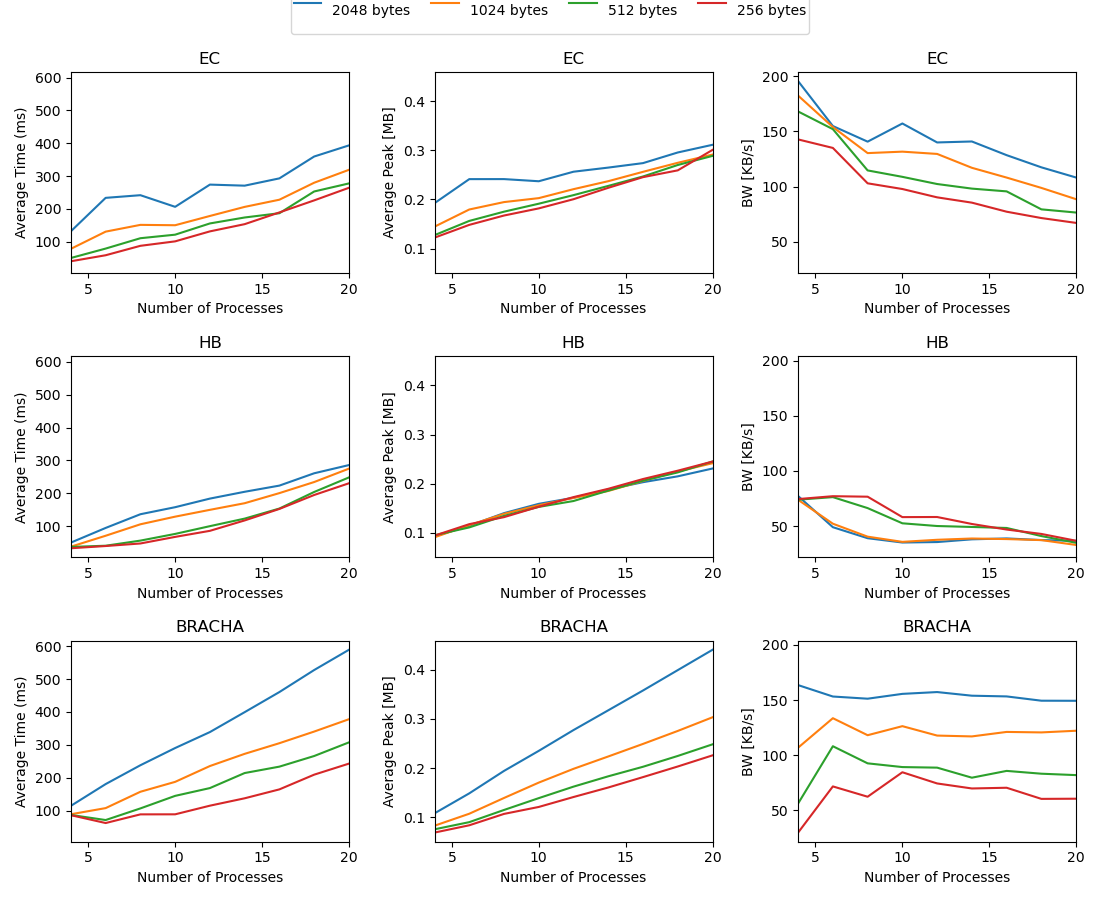
\includegraphics[scale=0.4]{LINE-GRAPH-3FINAL-2MBPS.png}
\caption{2MBPS}
\label{fig:mesh1}
\end{figure}
\\
The second picture compares the three protocols and it shows that the fastest protocol is always the HB protocol in terms of elapsed time while the EC is faster than the BRACHA for payload lengths smaller than 2048 bytes.\\
For the second evaluation metric we note that HB is the cheaper in terms of resources for 2048 and 1024 bytes but for smaller payloads the BRACHA implementation consumes a smaller portion of memory than HB. When the payload length reaches 2048 bytes the BRACHA implementation is the most expensive one; instead for smaller payloads the EC implementation makes use of a larger portion of memory.\\
HB implementation outperforms both Bracha and EC implementations in terms of bandwidth, because it transmits packets of fixed length.\\
\begin{figure}
\centering
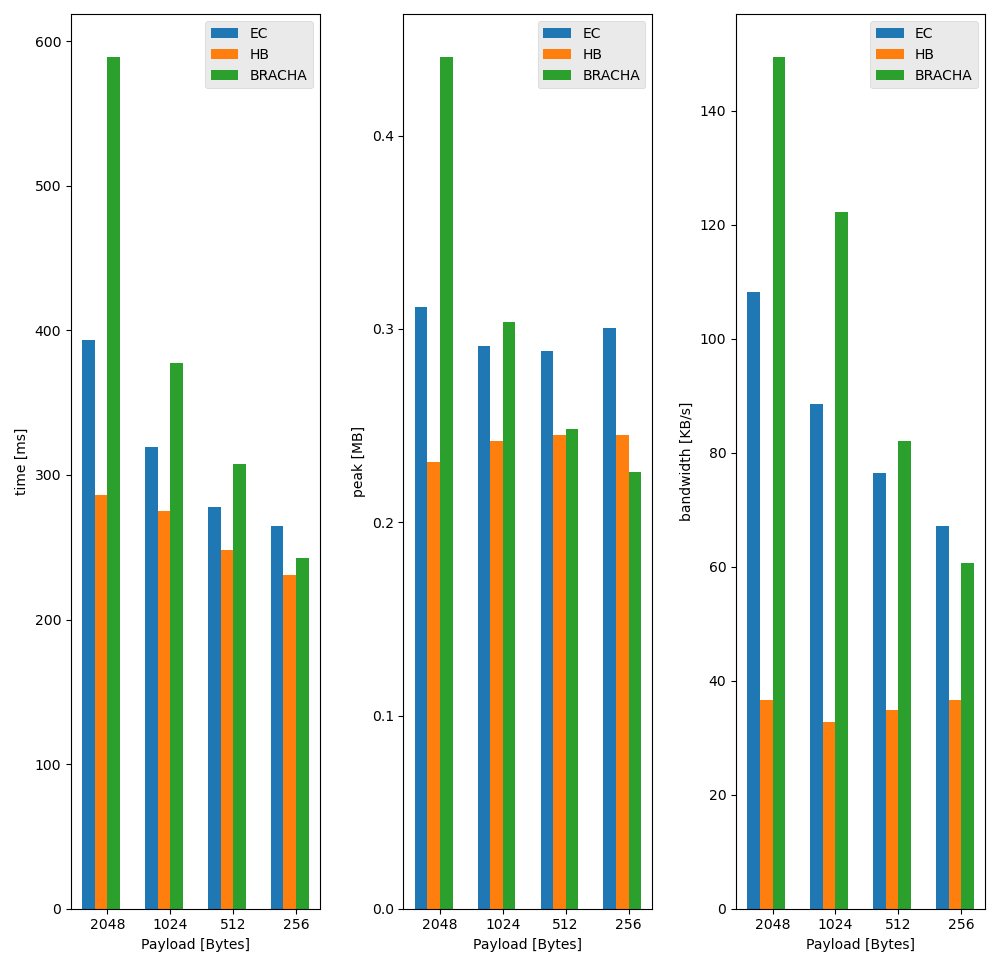
\includegraphics[scale=0.4]{BAR-GRAPH-3FINAL-2MBPS.png}
\caption{2MBPS}
\label{fig:mesh2}
\end{figure}
\\
The third picture show that HB is still the best protocol for all the three metrics. With limited bandwidth (500KBPS), EC and HB outperform Bracha in terms of time of a factor up to 2x, when the payload reaches 2048 bytes. \\
The situation is slightly better for Bracha in terms of memory usage, where for smaller payloads it becomes better than EC protocol, but still worse than HB one.\\
In terms of bandwidth, HB implementation outperforms both EC and Bracha ones, that use almost the same amount.\\ 
\begin{figure}
\centering
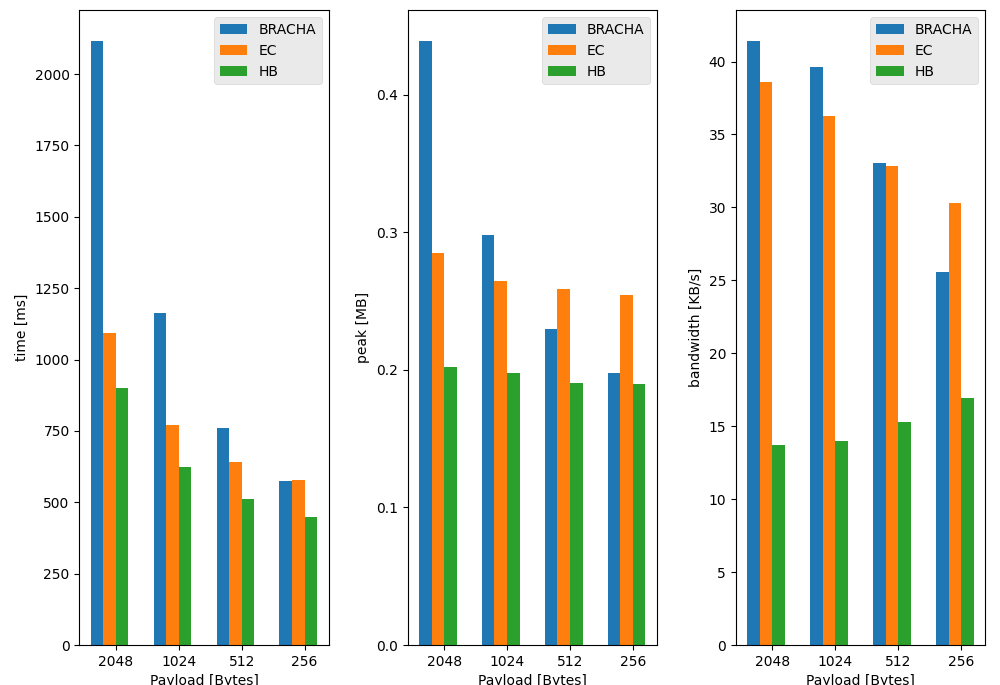
\includegraphics[scale=0.4]{BAR-BW-500KB-20-proc.png}
\caption{500KBPS}
\label{fig:mesh3}
\end{figure}
\\
In Figure 4, we also take into account AM implementation, although it is not comparable yet with others. \\
The first three implementations have been discussed above (HB, EC, Bracha). \\
AM implementation is outperformed by all other implementations of a factor 2x, in the best case (for payload size of 256 bytes), that reaches 10x for payload size of 2048 bytes, by considering all the metrics. \\
\begin{figure}
\centering
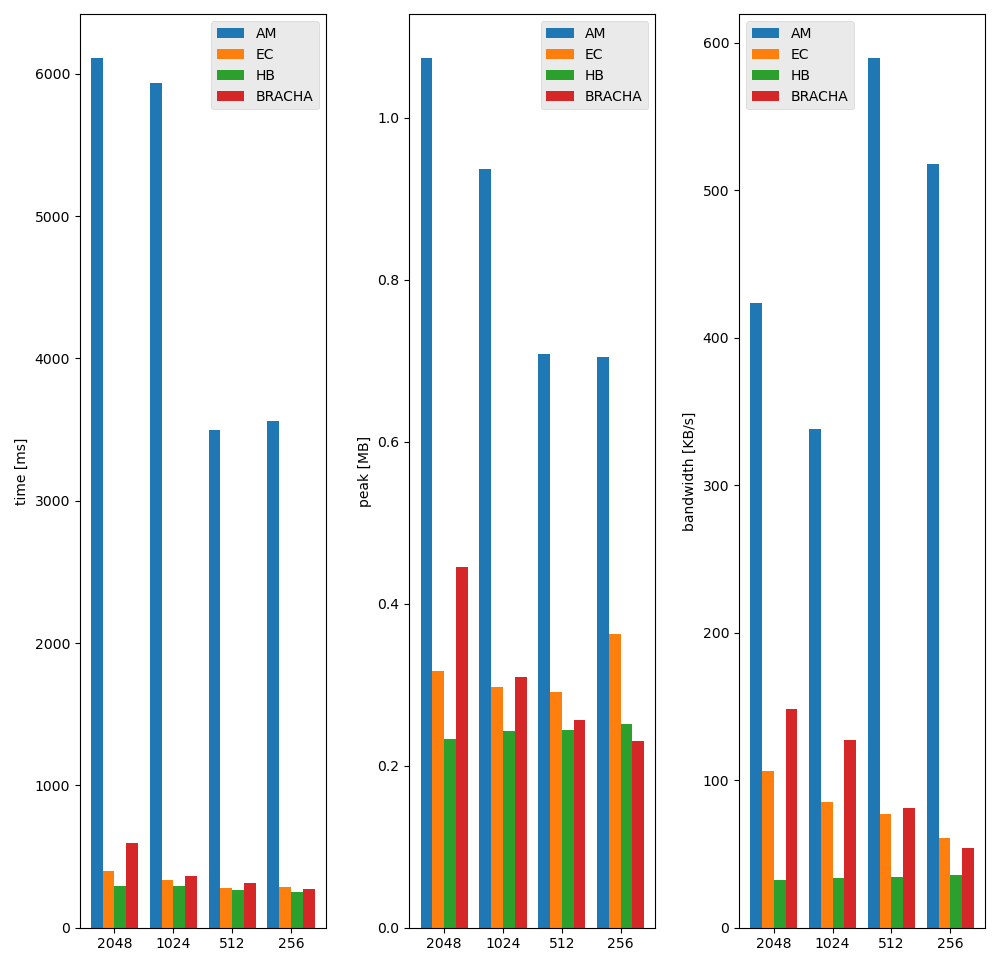
\includegraphics[scale=0.4]{BAR-BW-2MB-20-proc.png}
\caption{2MBPS}
\label{fig:mesh4}
\end{figure}
\\
In Figure 5, the bandwidth is increased up to 1GBPS. \\
In this case, AM implementation can be considered as an alternative to other protocols because its elapsed time is comparable; HB and Bracha implementations have similar performances in terms of execution time.\\
HB implementation outperforms others in terms of memory usage.\\
\begin{figure}
\centering
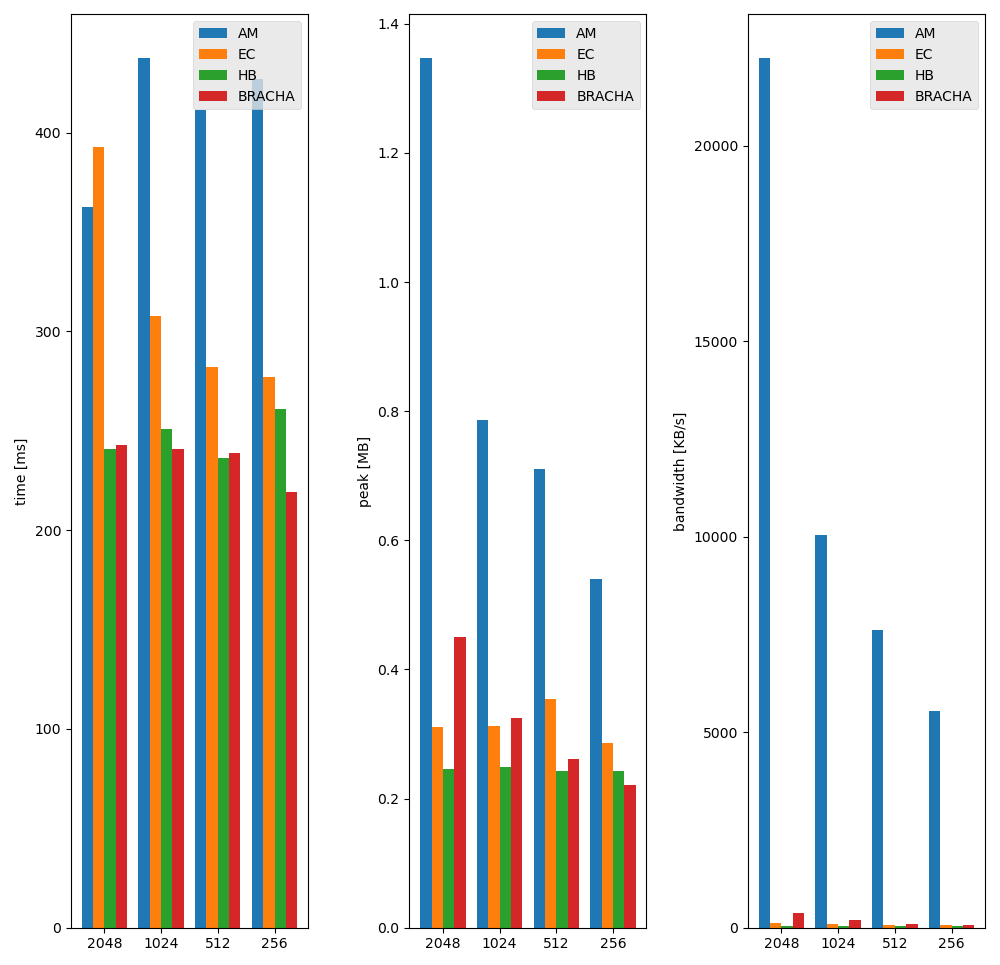
\includegraphics[scale=0.4]{BAR-BW-1GB-20-proc.png}
\caption{1GBPS}
\label{fig:mesh5}
\end{figure}
\\
In the sixth figure, Byzantine entities are introduced: they forge a new message whenever the protocol requires them to send something.\\
The results are not very different from the situation without them: indeed, the HB implementation is still the best one for all the metrics, while EC implementation performs better than Bracha when the payload is bigger and the situation reverts for smaller payloads. \\
\begin{figure}
\centering
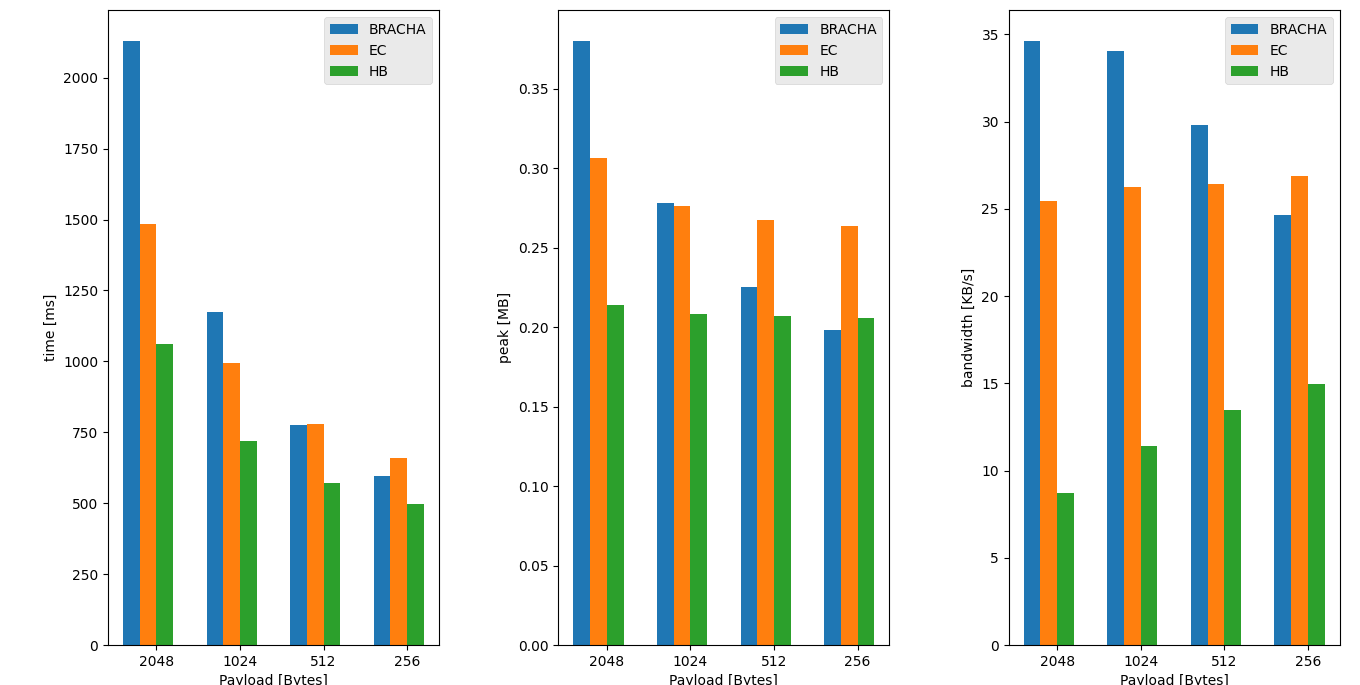
\includegraphics[scale=0.4]{BAR-4BYZ-BW-500KB-20-proc.png}
\caption{6BYZ-500KBPS}
\label{fig:mesh6}
\end{figure}
\\
In the last figure, the bandwidth is increased with respect to the previous evaluation, but Byzantine entities are still present. \\
In this case, Bracha implementation performs better than other ones in terms of execution time, while HB implementation performs slighty better in terms of both memory usage and bandwidth.\\
\begin{figure}
\centering
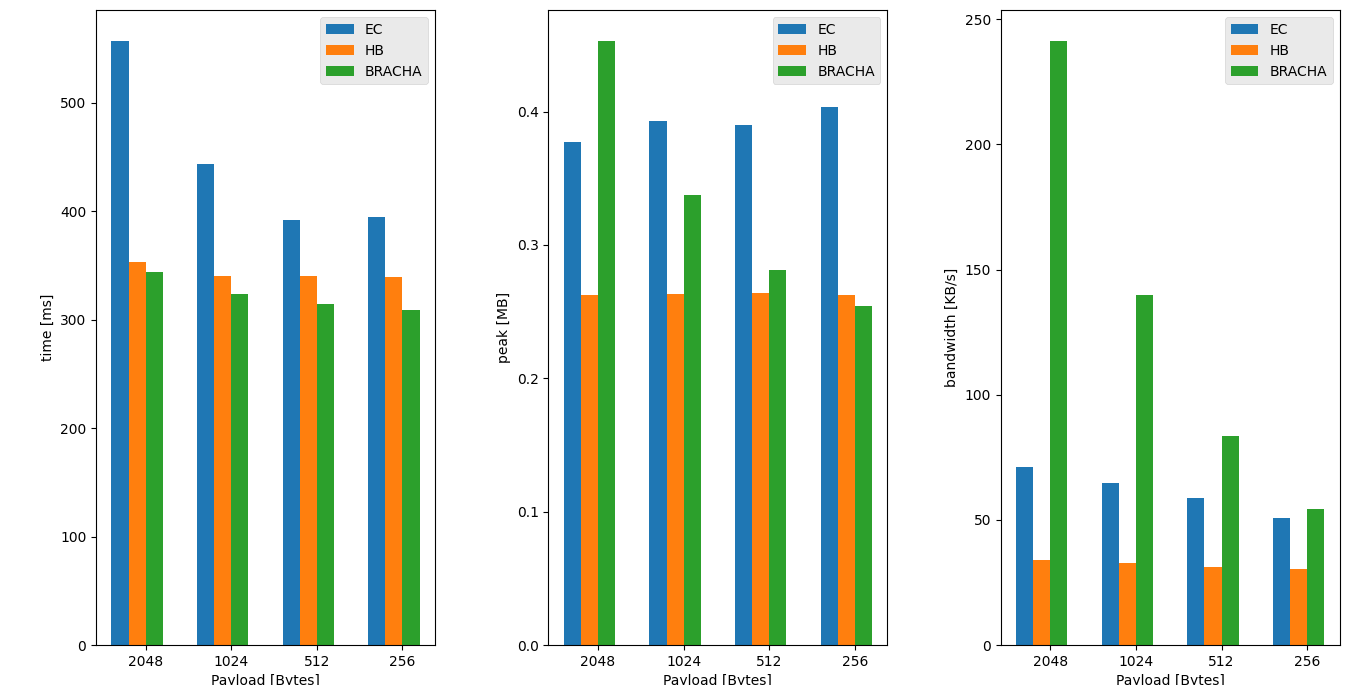
\includegraphics[scale=0.4]{BAR-BYZ-BW-10MBPS-20.png}
\caption{6BYZ-10MBPS}
\label{fig:mesh7}
\end{figure}

\newpage

\subsection{Conclusions}
In the average case, HB is the best protocol thanks to the hashing function that reduces all messages to a fixed length. If the number of processes, the bandwidth and the payload of each message (and consequently, the data exchanged between processes) are limited, the BRACHA protocol is the most efficient one.
When there is an high number of faulty processes (it does not matter if they are byzantine or just faulty) or there are no constraints on the bandwidth, the EC protocol is the one that obtains the best performances (although, in the case of unlimited bandwidth, the difference with HB is not so relevant). \\
Because of the cryptographic primitives used by the protocol, AM is not comparable with respect to the other protocols in terms of all the metrics defined in the evaluation. 
If for any reason an application needs the non repudiation requirement as a principal goal, the AM protocol meets the needs perfectly and it is the preferred one to use among all the four protocols evaluated.
Furthermore the implementation of the protocol is easier for the restricted number of protocol messages issued and  it is also much more understandable in terms of the specification description. 
The overall number of messages exchanged by the protocol is less than other protocols.
The elapsed time of the protocol is bounded to the last phase of the algorithm where there is an high number of steps for the verification of the n-f messages received; furthermore, the protocol uses a third entity (KDS) to distribute the keys needed for the cryptographic primitives that leads to higher delays.
Because of the reasons stated above, the following evaluation is centered on the remaining three protocols.
Protocols that send all the payload are better wrt the others if the payload size is small; when the payload increases, the Erasure-Code and Hash-Based protocols are better than the Bracha one because they send a smaller packet. The erasure code protocol sends the shares of the message and although they are smaller than the message they are longer than the hash; so hash based is the best among the four protocols. Furthermore Bracha has a simpler implementation and the overall number of messages exchanged is smaller than the other protocols.
Hash-Based remains the best because of the crypto hashing function that bounds the length of the payload to a fixed length, independently from the message size.
\end{document}
